% GENERATED FROM typst/manual/appendices/B_quarantined_external_comparison.typ BY scripts/typ2tex.py (v1.0.0) — DO NOT EDIT.
% Edit canonical Typst under typst/ and regenerate with: python3 scripts/typ2tex.py --root . --outdir latex

\section{Quarantined External Comparison}\label{manual:external-comparison}

\paragraph{Calculation card.}
The candidate rate, measured target energy and measured normalizer have
separate roles; $h_{\mathrm{ext}}$ and $e$ are defining constants.
The declared unit/rate maps produce the inline Tau target coordinates.
Their normalizer is shared across forward and inverse maps. The audit below
checks comparison order and units; physical prediction still needs a bound
candidate and its uncertainty under \secref{manual:calculation-spine}.

\subsection{Scope}\label{manual:external-comparison:scope}

This appendix compares A$\Omega$ outputs against external comparison coordinates. It does not import external units, constants, or symbols into the A$\Omega$ calculation. The active calculation produces a candidate such as

\[
\nu_{x,\AO}.
\]

Only after that value is declared may an external comparison record use it:

\[
\Qext(\nu_{x,\AO};\mathcal{T}_x).
\]

\subsection{Presentation-numeric policy}\label{manual:external-comparison:presentation-numeric-policy}

A$\Omega$-internal arithmetic remains integer/rational. The decimals in this appendix are external comparison presentation values. Measured external values are carried with a declared uncertainty; exact defining constants are marked as exact. The external normalizer $\eta_{\mathrm{ext}}$ is measured, so uncertainty propagation for normalized rates may include both the target-energy uncertainty and the uncertainty of $\eta_{\mathrm{ext}}$.

\subsection{External comparison symbols}\label{manual:external-comparison-symbols}

External constants and measured-sector units are named only inside this quarantine. The active A$\Omega$ notation is unaffected by them.

\subsubsection{Distance comparison}

If a bip duration $\Delta t_{\mathrm{bip}}$ is declared, an external distance coordinate may be recorded as

\[
d_{\mathrm{ext}}=c\,n\,\Delta t_{\mathrm{bip}},\qquad n\in\mathbb{Z}_{\ge0}.
\]

Here $c$ is an external defining constant in the comparison coordinate system.

\subsubsection{Speed comparison}

The active calculation may carry the exact integer pair

\[
(\Delta q,\Delta n),\qquad0\le\Delta q\le\Delta n,\qquad\Delta n>0.
\]

The external speed coordinate is allowed only after the integer pair is declared:

\[
\beta_{\mathrm{ext}}=\frac{\Delta q}{\Delta n},\qquad v_{\mathrm{ext}}=\beta_{\mathrm{ext}}c.
\]

\subsubsection{Direction comparison}

A direction comparison may record cycle count

\[
N_{\theta}=\frac{\Theta}{2\pi},\qquad2\pi\mapsto1\,\mathrm{cycle},\qquad4\pi\mapsto2\,\mathrm{cycles},
\]

with an orientation sign

\[
s_{\theta}\in\{-1,+1\}.
\]

\subsubsection{Charge comparison}

The active calculation carries integer orientation. The external charge coordinate may be recorded as

\[
Q_{\mathrm{ext}}=ze,\qquad z\in\mathbb{Z},
\]

where $e$ is an external defining constant in the comparison coordinate system.

\subsection{Choice: external rate normalizer}\label{manual:external-comparison:action-normalization}

Define the quarantined external rate normalizer

\[
\eta_{\mathrm{ext}}:=\alpha_{\mathrm{fs}}^{-1}.
\]

Use

\[
\alpha_{\mathrm{fs}}^{-1}=137.035999177(21)
\]

inside this appendix only. This symbol is external and does not set active A$\Omega$ notation.

Define the external comparison coefficient

\[
K_{\mathrm{ext}}=\frac{h_{\mathrm{ext}}\eta_{\mathrm{ext}}}{10^6e}=5.6673535511200\times10^{-19}\,\mathrm{MeV}\,\mathrm{s}.
\]

The uncertainty inherited from $\eta_{\mathrm{ext}}$ is

\[
\sigma_{K,\eta}=8.68490216354\times10^{-29}\,\mathrm{MeV}\,\mathrm{s}.
\]

Here $h_{\mathrm{ext}}$ and $e$ are external exact defining constants, while $\eta_{\mathrm{ext}}$ is measured. The active A$\Omega$ calculation does not use them.

Given a numeric A$\Omega$ candidate $\nu_{x,\AO}$, the external energy-coordinate comparison is

\[
E_{x,\mathrm{ext}}[\mathrm{MeV}]=K_{\mathrm{ext}}\nu_{x,\AO}.
\]

\subsection{Tau target record}\label{manual:external-comparison:tau-target-normalization}

The measured-comparison record in \secref{manual:rest:measured-comparison-analysis}, \tabref{tab:manual-measured-comparison-analysis}, uses the measured target

\[
E_{\tau}^{\mathrm{tar}}=1776.86\,\mathrm{MeV},\qquad\sigma_E=0.12\,\mathrm{MeV}.
\]

The target in the external joule coordinate is

\[
E_{\tau,J}^{\mathrm{tar}}=1776.86\times10^6e=2.84684357388924\times10^{-10}\,\mathrm{J}.
\]

The external frequency coordinate is

\[
f_{\tau}=\frac{E_{\tau,J}^{\mathrm{tar}}}{h_{\mathrm{ext}}}=4.2964283646910\times10^{23}\mathrm{s}^{-1}.
\]

The quarantined external target rate is

\[
\nu_{\tau,\mathrm{tar}}=\frac{f_{\tau}}{\eta_{\mathrm{ext}}}=3.1352552544544\times10^{21}\mathrm{s}^{-1}.
\]

The target-energy contribution to the external target-rate uncertainty is

\[
\sigma_{\nu,E}=\frac{0.12\times10^6e}{h_{\mathrm{ext}}\eta_{\mathrm{ext}}}=2.11739039955\times10^{17}\mathrm{s}^{-1}.
\]

The contribution from the measured external normalizer is

\[
\sigma_{\nu,\eta}=\nu_{\tau,\mathrm{tar}}\frac{0.000000021}{137.035999177}=4.80460322389\times10^{11}\mathrm{s}^{-1}.
\]

At first order, assuming zero covariance between the target energy and
measured normalizer, the combined external target-rate uncertainty is

\[
\sigma_{\nu,\mathrm{comb}}=\sqrt{\sigma_{\nu,E}^2+\sigma_{\nu,\eta}^2}=2.11739039956\times10^{17}\mathrm{s}^{-1}.
\]

\begin{table}[H]
\centering
\caption{Tau target record in the quarantined external-comparison coordinate.}
{\footnotesize
\begin{tabularx}{\linewidth}{c>{\raggedright\arraybackslash}Xcc}
\toprule
$x$ & $\operatorname{def}(x)$ & $\operatorname{val}(x)$ & $\operatorname{unit}(x)$ \\
\midrule
$E_{\tau}^{\mathrm{tar}}$ & declared measured target & $1776.86$ & $\mathrm{MeV}$ \\
$\sigma_E$ & declared uncertainty & $0.12$ & $\mathrm{MeV}$ \\
$E_{\tau,J}^{\mathrm{tar}}$ & $1776.86\times10^6e$ & $2.84684357388924\times10^{-10}$ & $\mathrm{J}$ \\
$f_{\tau}$ & $E_{\tau,J}^{\mathrm{tar}}/h_{\mathrm{ext}}$ & $4.2964283646910\times10^{23}$ & $\mathrm{s}^{-1}$ \\
$\eta_{\mathrm{ext}}$ & $\alpha_{\mathrm{fs}}^{-1}$ & $137.035999177(21)$ & $1$ \\
$\nu_{\tau,\mathrm{tar}}$ & $f_{\tau}/\eta_{\mathrm{ext}}$ & $3.1352552544544\times10^{21}$ & $\mathrm{s}^{-1}$ \\
$\sigma_{\nu,E}$ & energy uncertainty contribution & $2.11739039955\times10^{17}$ & $\mathrm{s}^{-1}$ \\
$\sigma_{\nu,\eta}$ & normalizer uncertainty contribution & $4.80460322389\times10^{11}$ & $\mathrm{s}^{-1}$ \\
$\sigma_{\nu,\mathrm{comb}}$ & combined uncertainty & $2.11739039956\times10^{17}$ & $\mathrm{s}^{-1}$ \\
$K_{\mathrm{ext}}$ & $h_{\mathrm{ext}}\eta_{\mathrm{ext}}/(10^6e)$ & $5.6673535511200\times10^{-19}$ & $\mathrm{MeV}\,\mathrm{s}$ \\
$\sigma_{K,\eta}$ & normalizer contribution to $K_{\mathrm{ext}}$ & $8.68490216354\times10^{-29}$ & $\mathrm{MeV}\,\mathrm{s}$ \\
\bottomrule
\end{tabularx}
}
\end{table}

Using the identical quarantined normalizer $K_{\mathrm{ext}}=h_{\mathrm{ext}}\eta_{\mathrm{ext}}/(10^6e)$, the reference engine (\texttt{manual/data/boundary\_sadar/rest\_energy\_sadar\_debris\_atlas.csv}, vector \texttt{SD-007}) evaluates the exact rational target rates $\nu_{x,\mathrm{tar}}=E_x^{\mathrm{tar}}/K_{\mathrm{ext}}$ across all nine rest-energy target records ($0.000902$, $0.186433$, $3.135255$, $9.315477$, $9.316024$, $9.469905$, $11.071252$, $1.655574$, and $1.657856$ in units of $10^{21}\,\mathrm{s}^{-1}$ for $e^-$, $\mu^-$, $\tau^-$, $B^{\pm}$, $B^0$, $B_s^0$, $B_c^{\pm}$, $p^+$, and $n^0$), keeping SI defining constants and CODATA/PDG targets strictly inside $B_{\mathrm{ext}}$.

\subsection{Audit}\label{manual:external-comparison:falsification}

The same normalizer identity must be retained in a round trip:
$K_{\mathrm{ext}}\nu_{\tau,\mathrm{tar}}=E_{\tau}^{\mathrm{tar}}$.
Its uncertainty cancels exactly in this algebraic composition. Treating
the two appearances of $\eta_{\mathrm{ext}}$ as independent would add a
spurious contribution; the joint route of
\secref{manual:scoped-errors-data-support} preserves that dependence.

F1. External-comparison audit records the active $\nu_{x,\AO}$ candidate before the external comparison.

F2. Speed-comparison audit records integer $\Delta q$, integer positive $\Delta n$, and $\Delta q\le\Delta n$.

F3. Direction-cycle audit records direction relative to $2\pi=1$ cycle.

F4. Charge-comparison audit records integer orientation before the external charge comparison.

F5. Quarantine audit records external constants, units, and measured-sector symbols only after the active A$\Omega$ calculation.

\aodprovenance{\mainequation{main:eq:b-scoped-flux};
\mainequation{main:eq:sadar-attention-vector};
\secref{manual:exact-arithmetic-presentation};
\secref{manual:external-comparison-quarantine}.}

\aodliteraturenote{SI defining constants: BIPM~\cite{bipm-si-defining-constants}, inverse fine-structure constant: NIST CODATA~\cite{nist-alpha-inverse}, tau target: Zhang/PDG~\cite{zhang-tau-pdg}, DESY/Belle~\cite{desy-belle-tau}.}

\aodremark{The quarantined external-comparison appendix compares against A$\Omega$ outputs. It does not import external constants or symbols into the A$\Omega$ calculation.}

\subsection{Five-boundary \texorpdfstring{$\mathsf{Q}_{\mathrm{ext}}$}{Qext} firewall and six-tuple precision ledger}\label{manual:qext:dec-quarantine-firewall}

At the terminal boundary $B_{\mathrm{ext}}=\mathsf{Q}_{\mathrm{ext}}(\nu_{x,\AO};\mathcal{T}_x)$ of every five-boundary stack, native $\mathbb{Z}/\mathbb{Q}$ invariants from \secref{manual:rest-energy-prediction} --- verified by vectors \texttt{RC-027} (Tau $1:2:9_{\mathrm{yro}}$ $50$-microslot rotor and shedding trace), \texttt{RC-028} (core-starvation $3:2$ Ditrion debris ladder and $3:3:7_{\mathrm{yro}}$ Higgs midpoint saddle), and \texttt{RC-029} (ten-carrier rest-energy atlas, $8160$ bit-window span versus $9104$ summed lineage closures) --- project one-way into six-tuple precision records $(x_{\mathrm{disp}},u_x,\operatorname{unit}(x),\operatorname{src}(x),\operatorname{round}(x),\operatorname{scope}(x))$. External target-rate normalization and exact round-trip $\eta_{\mathrm{ext}}$ cancellation across all nine rest-energy target records are verified by vector \texttt{SD-007} (\texttt{manual/data/boundary\_sadar/rest\_energy\_sadar\_debris\_atlas.csv}), while post-freeze exact rational half-even six-decimal Higgs LHC comparison displays and rounding residuals are verified by vectors \texttt{SD-004} and \texttt{SD-005}. In the round-trip expression $\nu_{\mathrm{sc}}=\nu_{\AO}/\eta_{\mathrm{ext}}$ followed by $E_{\mathrm{map}}=K_{\mathrm{ext}}\eta_{\mathrm{ext}}\nu_{\mathrm{sc}}=K_{\mathrm{ext}}\nu_{\AO}$, the external constant $\eta_{\mathrm{ext}}=\alpha_{\mathrm{fs}}^{-1}$ cancels identically and adds zero native degrees of freedom. Under standing R04 S3 discipline, simulation-substrate and computational-calculus equivalence claims remain permanently quarantined outside Main ontology and native Manual derivations.

\begin{figure}[H]
\centering
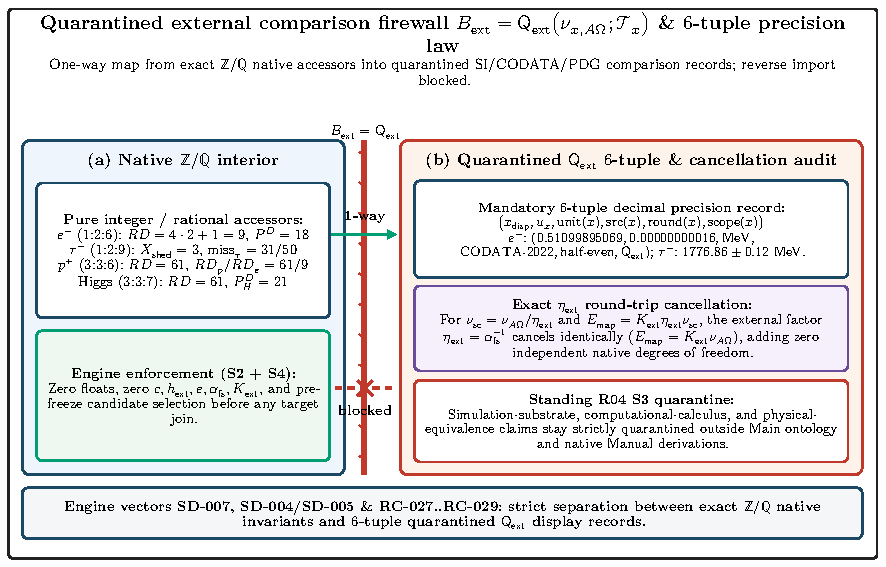
\includegraphics[width=0.92\linewidth,height=0.78\textheight,keepaspectratio]{figures/generated/qext-quarantine-firewall.pdf}
\caption{Quarantined external comparison firewall $B_{\mathrm{ext}}=\mathsf{Q}_{\mathrm{ext}}(\nu_{x,\AO};\mathcal{T}_x)$, six-tuple decimal precision record, exact $\eta_{\mathrm{ext}}$ cancellation, and standing R04 S3 quarantine (\texttt{SD-007}, \texttt{rest\_energy\_sadar\_debris\_atlas.csv}).}
\label{fig:manual-qext-quarantine-firewall}
\end{figure}

\begin{table}[H]
\centering
\caption{Six-tuple quarantined $\mathsf{Q}_{\mathrm{ext}}$ target-precision records paired with exact native support accessors (\texttt{SD-007}, \texttt{SD-004}, \texttt{SD-005}, \texttt{RC-027}--\texttt{RC-029}).}
\label{tab:manual-qext-precision-ledger}
{\footnotesize
\begin{tabular}{>{\raggedright\arraybackslash}p{0.072\linewidth}>{\raggedright\arraybackslash}p{0.144\linewidth}>{\raggedleft\arraybackslash}p{0.128\linewidth}>{\raggedleft\arraybackslash}p{0.128\linewidth}>{\centering\arraybackslash}p{0.072\linewidth}>{\raggedright\arraybackslash}p{0.160\linewidth}>{\raggedright\arraybackslash}p{0.096\linewidth}}
\toprule
Carrier & Native $M_x$ ($RD$) & $x_{\mathrm{disp}}$ & $u_x$ & Unit & Source & Scope \\
\midrule
$e^-$ & $1:2:6$ ($9$) & 0.51099895069 & 0.00000000016 & MeV & CODATA-2022 & $\mathsf{Q}_{\mathrm{ext}}$ \\
$\mu^-$ & $1:2:8$ ($9$) & 105.6583755 & 0.0000023 & MeV & CODATA-2022 & $\mathsf{Q}_{\mathrm{ext}}$ \\
$\tau^-$ & $1:2:9_{\mathrm{yro}}$ ($9$) & 1776.86 & 0.12 & MeV & PDG-2024 & $\mathsf{Q}_{\mathrm{ext}}$ \\
$p^+$ & $3:3:6$ ($61$) & 938.27208943 & 0.00000029 & MeV & CODATA-2022 & $\mathsf{Q}_{\mathrm{ext}}$ \\
$n^0$ & $3:4:6$ ($137$) & 939.56542194 & 0.00000048 & MeV & CODATA-2022 & $\mathsf{Q}_{\mathrm{ext}}$ \\
Higgs & $3:3:7_{\mathrm{yro}}$ ($61$) & 125090 & 240 & MeV & ATLAS+CMS Run-1 & $\mathsf{Q}_{\mathrm{ext}}$ \\
\bottomrule
\end{tabular}
}
\end{table}
